\documentclass[border=10pt]{standalone} 
\usepackage[utf8]{inputenc}
\usepackage{nacal}
\usepackage{pgfplots}
\usepackage{tikz-3dplot}
\usepackage{tikz} 
\usetikzlibrary{matrix,decorations.pathreplacing}
\usetikzlibrary{calc,angles,positioning,intersections,quotes,decorations.markings}
\usepackage{tkz-euclide}

\pgfplotsset{width=10cm,height=6cm}

\begin{document}
  \def\Rojo{red!50!black}
  \def\RojoOscuro{red!20!black}
  \def\RojoClaro{red!90!black}
  \def\Verde{green!50!black}
  \def\VerdeOscuro{green!30!black}
  \def\VerdeClaro{green!50!gray}
  \def\Azul{blue!50!black}
  \def\AzulOscuro{blue!35!black}
  \def\AzulClaro{blue!60!gray}

  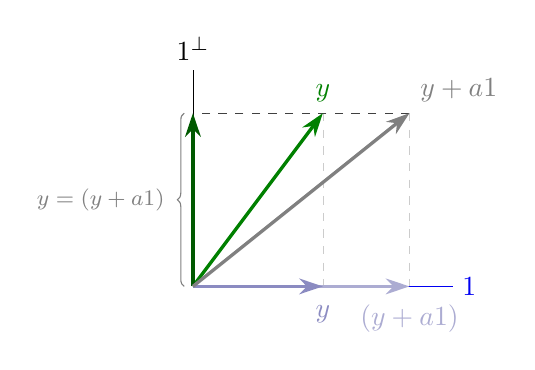
\begin{tikzpicture}[scale=1.1]
    % vértices del triángulo
    \coordinate (v1) at (0,0);
    \coordinate (v2) at (3,0); % punta eje horizontal
    \coordinate (v3) at (1.5,2);
    
    \coordinate (v4) at (1.5,0);  
    
    \coordinate (v6) at (0,2); % vector e
    \coordinate (v7) at (0,2.5); % punta eje vertical
    
    \coordinate (v8) at (2.5,2);
    \coordinate (v9) at (2.5,0);  
    
    % division del triangulo
    \draw[-,gray!40,dashed,very thin]  (v3) -- (v4);
    \draw[-,gray!50!black,dashed,very thin]  (v8) -- (v6);
    \draw[-,gray!40,dashed,very thin]  (v8) -- (v9);
    
    \draw[color=blue!95!black,very thin]  (v1) -- (v2) node [right]  {$\Span{\Vect{1}}$};
    \draw[very thin]  (v1) -- (v7) node [above]  {$\Span{\Vect{1}}^\perp$};
    \draw[-{Stealth[length=3mm, width=2mm]},very thick,green!50!black] (v1) -- (v3) node [above]  {$\Vect{y}$};
    
    \draw[-{Stealth[length=3mm, width=2mm]},very thick,gray!70!blue!50] (v1) -- (v9) node [below,yshift=-1mm]  {$\Media{(\Vect{y}+a\Vect{1})}$};
    \draw[-{Stealth[length=3mm, width=2mm]},very thick,gray!70!blue!70] (v1) -- (v4) node [below,yshift=-1mm]  {$\Vect{\Media{y}}$};
    \draw[-{Stealth[length=3mm, width=2mm]},very thick,green!35!black] (v1) -- (v6); % node [left,xshift=-1mm]   {$\Vect{y}-\Vect{\Media{y}}=\Vect{e}$};
    
    \draw[decorate, decoration={brace},gray] (-0.1,0) -- (-0.1,2) node [midway, anchor=east, xshift=-1mm, outer sep=1pt,font=\footnotesize]{$\dt{\Vect{y}}=\dt{(\Vect{y}+a\Vect{1})}$};

    \draw[-{Stealth[length=3mm, width=2mm]},very thick, gray] (v1) -- (v8) node [anchor=south west]  {$\Vect{y}+a\Vect{1}$};
    
  \end{tikzpicture} 
\end{document}
